\documentclass[final,xcolor={usenames,x11names}]{beamer}
\usepackage[usenames,x11names]{xcolor,colortbl}
\usepackage[utf8]{inputenc}
\usepackage{cite}
%\usepackage[cmex10]{amsmath}
%%\interdisplaylinepenalty=2500
\usepackage{tikz}
\usepackage{pgf-umlcd}
\usepackage{algorithmic}
\usepackage{array}
\usepackage{url}
\usepackage{mathtools}
\hyphenation{op-tical net-works semi-conduc-tor method methods}
\usepackage{float}
\usepackage[scale=0.8]{beamerposter}
\usetheme{confposter}

\renewcommand*\rmdefault{ppl}

%\ifCLASSOPTIONcompsoc
%  \usepackage[caption=false,font=normalsize,labelfont=sf,textfont=sf]{subfig}
%\else
%  \usepackage[caption=false,font=footnotesize]{subfig}
%\fi

%\ifCLASSINFOpdf
%  \usepackage[pdftex]{graphicx}
  % declare the path(s) where your graphic files are
  % \graphicspath{{../pdf/}{../jpeg/}}
  % and their extensions so you won't have to specify these with
  % every instance of \includegraphics
%  \DeclareGraphicsExtensions{.pdf,.jpeg,.jpg,.png}
%\else
  % or other class option (dvipsone, dvipdf, if not using dvips). graphicx
  % will default to the driver specified in the system graphics.cfg if no
  % driver is specified.
%  \usepackage[dvips]{graphicx}
  % declare the path(s) where your graphic files are
  % \graphicspath{{../eps/}}
  % and their extensions so you won't have to specify these with
  % every instance of \includegraphics
%  \DeclareGraphicsExtensions{.eps}
%\fi

\floatstyle{ruled}
\newfloat{json}{thp}{lop}
\floatname{program}{Program}

\newlength{\sepwid}
\newlength{\onecolwid}
\newlength{\twocolwid}
\newlength{\threecolwid}
\setlength{\paperwidth}{48in} % A0 width: 46.8in
\setlength{\paperheight}{36in} % A0 height: 33.1in
\setlength{\sepwid}{0.01\paperwidth} % Separation width (white space) between columns
\setlength{\onecolwid}{0.30\paperwidth} % Width of one column
\setlength{\twocolwid}{0.6\paperwidth} % Width of two columns
\setlength{\threecolwid}{0.9\paperwidth} % Width of three columns
\setlength{\topmargin}{-0.5in} % Reduce the top margin size
\setlength{\arrayrulewidth}{2pt}

%opening
\title{FAS Simulator – Executive Summary}
\author{Tero Keski-Valkama}
\institute{Faculty of Computing and Electrical Engineering, Tampere University of Technology}

\begin{document}

\begin{frame}[t]

\begin{columns}[t]

\begin{column}{\sepwid}\end{column} % Empty spacer column

\begin{column}{\onecolwid}

\begin{alertblock}{Topic}

\begin{itemize}
\item Once upon a time, there was a factory.
\end{itemize}

{\centering
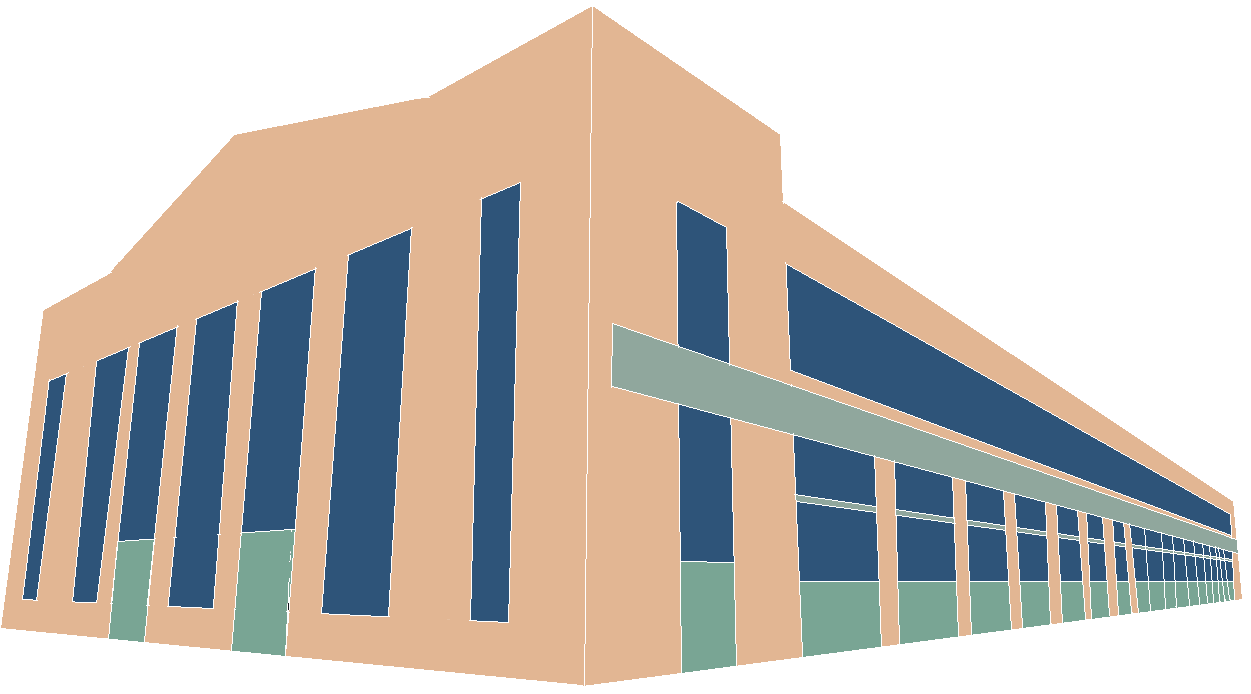
\includegraphics[width=8 cm,keepaspectratio=true]{./factory.png}\par
}

\begin{itemize}
\item The factory had a process.
\end{itemize}

{\centering
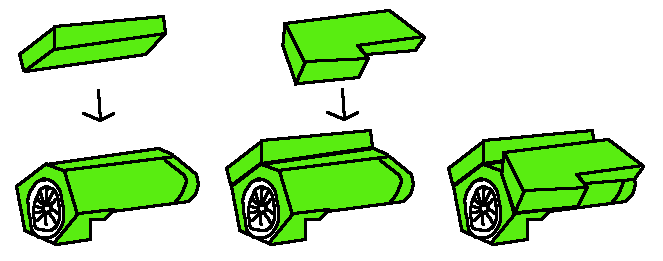
\includegraphics[width=8 cm,keepaspectratio=true]{./assembly.png}\par
}

\begin{itemize}
\item The process creates a log file.
\end{itemize}

\begin{center}
{
\ttfamily
\begin{tabular}{|c|}
  \hline
  \cellcolor{PaleTurquoise1}
Product moved to Workplace 1
  \\
  \hline
  \cellcolor{PaleTurquoise1}
Part A attached to Product
  \\
  \hline
  \cellcolor{PaleTurquoise1}
Product moved to Workplace 2
  \\
  \hline
  \cellcolor{PaleTurquoise1}
Part B attached to Product
  \\
  \hline
  \cellcolor{PaleTurquoise1}
Product moved to Workplace 3
  \\
  \hline
  \cellcolor{PaleTurquoise1}
Product tested
  \\
  \hline
\end{tabular}
}
\end{center}

\begin{itemize}
\item Multiple products are going through the factory at the same time.
\item The log becomes interlaced.
\end{itemize}

\begin{center}
{
\ttfamily
\begin{tabular}{|c|}
  \hline
  \cellcolor{PaleTurquoise1}
Product moved to Workplace 1
  \\
  \hline
  \cellcolor{PaleTurquoise1}
Part A attached to Product
  \\
  \hline
  \cellcolor{PaleTurquoise1}
Product moved to Workplace 2
  \\
  \hline
  \cellcolor{PaleTurquoise1>wheel,1,5}
Product moved to Workplace 1
  \\
  \hline
  \cellcolor{PaleTurquoise1>wheel,1,5}
Part A attached to Product
  \\
  \hline
  \cellcolor{PaleTurquoise1}
Part B attached to Product
  \\
  \hline
  \cellcolor{PaleTurquoise1}
Product moved to Workplace 3
  \\
  \hline
  \cellcolor{PaleTurquoise1>wheel,1,5}
Product moved to Workplace 2
  \\
  \hline
  \cellcolor{PaleTurquoise1>wheel,1,5}
Part B attached to Product
  \\
  \hline
  \cellcolor{PaleTurquoise1}
Product tested
  \\
  \hline
  \cellcolor{PaleTurquoise1>wheel,1,5}
Product moved to Workplace 3
  \\
  \hline
  \cellcolor{PaleTurquoise1>wheel,1,5}
Product tested
  \\
  \hline
\end{tabular}
}
\end{center}

\begin{itemize}
\item The factory owner adds an internet of things vibration sensors to the equipment, to get information when the equipment is started and stopped.
Additionally, there is a periodic clock-type event with periodic ticks unrelated to assembly.
\item These events are mixed into the logs along with the process events.
\end{itemize}

\begin{center}
{
\ttfamily
\begin{tabular}{|c|}
  \hline
  \cellcolor{PaleTurquoise1}
Product moved to Workplace 1
  \\
  \hline
  \cellcolor{PaleTurquoise1>wheel,2,5}
Equipment 1 started
  \\
  \hline
  \cellcolor{PaleTurquoise1>wheel,4,5}
Tick
  \\
  \hline
  \cellcolor{PaleTurquoise1>wheel,2,5}
Equipment 1 stopped
  \\
  \hline
  \cellcolor{PaleTurquoise1}
Part A attached to Product
  \\
  \hline
  \cellcolor{PaleTurquoise1>wheel,4,5}
Tick
  \\
  \hline
  \cellcolor{PaleTurquoise1}
Product moved to Workplace 2
  \\
  \hline
  \cellcolor{PaleTurquoise1>wheel,1,5}
Product moved to Workplace 1
  \\
  \hline
  \cellcolor{PaleTurquoise1>wheel,4,5}
Tick
  \\
  \hline
  \cellcolor{PaleTurquoise1>wheel,2,5}
Equipment 1 started
  \\
  \hline
  \cellcolor{PaleTurquoise1>wheel,2,5}
Equipment 1 stopped
  \\
  \hline
  \cellcolor{PaleTurquoise1>wheel,4,5}
Tick
  \\
  \hline
  \cellcolor{PaleTurquoise1>wheel,1,5}
Part A attached to Product
  \\
  \hline
  \cellcolor{PaleTurquoise1>wheel,2,5}
Equipment 2 started
  \\
  \hline
  \cellcolor{PaleTurquoise1>wheel,4,5}
Tick
  \\
  \hline
  \cellcolor{PaleTurquoise1>wheel,2,5}
Equipment 2 stopped
  \\
  \hline
  \cellcolor{PaleTurquoise1}
Part B attached to Product
  \\
  \hline
  \cellcolor{PaleTurquoise1}
Product moved to Workplace 3
  \\
  \hline
  \cellcolor{PaleTurquoise1>wheel,4,5}
Tick
  \\
  \hline
  \cellcolor{PaleTurquoise1>wheel,1,5}
Product moved to Workplace 2
  \\
  \hline
  \cellcolor{PaleTurquoise1>wheel,2,5}
Equipment 2 started
  \\
  \hline
  \cellcolor{PaleTurquoise1>wheel,4,5}
Tick
  \\
  \hline
  \cellcolor{PaleTurquoise1>wheel,2,5}
Equipment 2 stopped
  \\
  \hline
  \cellcolor{PaleTurquoise1>wheel,1,5}
Part B attached to Product
  \\
  \hline
  \cellcolor{PaleTurquoise1>wheel,4,5}
Tick
  \\
  \hline
  \cellcolor{PaleTurquoise1>wheel,4,5}
Tick
  \\
  \hline
  \cellcolor{PaleTurquoise1}
Product tested
  \\
  \hline
  \cellcolor{PaleTurquoise1>wheel,1,5}
Product moved to Workplace 3
  \\
  \hline
  \cellcolor{PaleTurquoise1>wheel,1,5}
Product tested
  \\
  \hline
\end{tabular}
}
\end{center}

\end{alertblock}
\end{column}

\begin{column}{\sepwid}\end{column} % Empty spacer column

\begin{column}{\onecolwid}
\begin{block}{Idea}

{\centering

\includegraphics[width=4 cm,keepaspectratio=true]{./bulb.png}\par
}

\begin{itemize}
\item If we had a learning system that can learn these kinds of processes from observing the logs, it could alert us if it sees something unexpected.
\item How can we support the design of a learning system that is adept at learning process models from symbolic logs?
\end{itemize}

\end{block}

\vspace{3cm}

\begin{alertblock}{Computer's View to the Log}

\begin{itemize}
\item As the computer does not know what events correspond to what products, the computer only sees the types of each event without knowing their meaning, like this:
\end{itemize}

\begin{center}
{
\ttfamily
\begin{tabular}{|c|}
  \hline
  \cellcolor{PaleTurquoise2}\hspace{3cm}
  \\
  \hline
  \cellcolor{PaleTurquoise2>wheel,1,11}\hspace{3cm}
  \\
  \hline
  \cellcolor{PaleTurquoise2>wheel,2,11}\hspace{3cm}
  \\
  \hline
  \cellcolor{PaleTurquoise2>wheel,3,11}\hspace{3cm}
  \\
  \hline
  \cellcolor{PaleTurquoise2>wheel,4,11}\hspace{3cm}
  \\
  \hline
  \cellcolor{PaleTurquoise2>wheel,2,11}\hspace{3cm}
  \\
  \hline
  \cellcolor{PaleTurquoise2>wheel,5,11}\hspace{3cm}
  \\
  \hline
  \cellcolor{PaleTurquoise2}\hspace{3cm}
  \\
  \hline
  \cellcolor{PaleTurquoise2>wheel,2,11}\hspace{3cm}
  \\
  \hline
  \cellcolor{PaleTurquoise2>wheel,1,11}\hspace{3cm}
  \\
  \hline
  \cellcolor{PaleTurquoise2>wheel,3,11}\hspace{3cm}
  \\
  \hline
  \cellcolor{PaleTurquoise2>wheel,2,11}\hspace{3cm}
  \\
  \hline
  \cellcolor{PaleTurquoise2>wheel,4,11}\hspace{3cm}
  \\
  \hline
  \cellcolor{PaleTurquoise2>wheel,6,11}\hspace{3cm}
  \\
  \hline
  \cellcolor{PaleTurquoise2>wheel,2,11}\hspace{3cm}
  \\
  \hline
  \cellcolor{PaleTurquoise2>wheel,7,11}\hspace{3cm}
  \\
  \hline
  \cellcolor{PaleTurquoise2>wheel,8,11}\hspace{3cm}
  \\
  \hline
  \cellcolor{PaleTurquoise2>wheel,9,11}\hspace{3cm}
  \\
  \hline
  \cellcolor{PaleTurquoise2>wheel,2,11}\hspace{3cm}
  \\
  \hline
  \cellcolor{PaleTurquoise2>wheel,5,11}\hspace{3cm}
  \\
  \hline
  \cellcolor{PaleTurquoise2>wheel,6,11}\hspace{3cm}
  \\
  \hline
  \cellcolor{PaleTurquoise2>wheel,2,11}\hspace{3cm}
  \\
  \hline
  \cellcolor{PaleTurquoise2>wheel,7,11}\hspace{3cm}
  \\
  \hline
  \cellcolor{PaleTurquoise2>wheel,8,11}\hspace{3cm}
  \\
  \hline
  \cellcolor{PaleTurquoise2>wheel,2,11}\hspace{3cm}
  \\
  \hline
  \cellcolor{PaleTurquoise2>wheel,2,11}\hspace{3cm}
  \\
  \hline
  \cellcolor{PaleTurquoise2>wheel,10,11}\hspace{3cm}
  \\
  \hline
  \cellcolor{PaleTurquoise2>wheel,9,11}\hspace{3cm}
  \\
  \hline
  \cellcolor{PaleTurquoise2>wheel,10,11}\hspace{3cm}
  \\
  \hline
\end{tabular}
}
\end{center}

\end{alertblock}

\vspace{10cm}

\begin{block}{From Simulators to Learning Systems}
All kinds of industrial and logistic processes create event logs. The events in these logs are created by different devices, and often we do not know
the explicit process model of the processes that create these events.

Wouldn't it be great if we could create a machine learning system that can observe these kinds of logs, and deduce the model of the process?

There are some existing methods for that, but those are very limited. Current methods can only extract an explicit process model
from logs when the process instance is identified for each event. The extracted process model is formal and definite and does not capture
an intuitive understanding of the process. The formal model only tells us which sequences are allowed and which are not allowed.

Modern machine learning methods can capture intuitive understanding and approximate facts of such processes. For example, a system can observe that the new vibration sensor added is related to the process
even if the vibration events are not matched one-to-one to a specific product.
\end{block}

\end{column}
\begin{column}{\sepwid}\end{column} % Empty spacer column

\begin{column}{\onecolwid}

\begin{alertblock}{Discrete Event Simulator}

\begin{itemize}
 \item A Discrete Event Simulator (DES) is a system which simulates a system in an event-oriented fashion.
 \item The system consists of component processes which wait and send events, and interact.
 \item The simulation output is a sequence of events and timestamps.
\end{itemize}


\end{alertblock}

\vspace{3cm}

\begin{block}{Simulator}

\begin{tikzpicture}
\begin{class}[text width=8cm]{FASInstance}{0,25}
\operation{+  spawn()}
\end{class}
\begin{class}[text width=8cm]{ProductionLine}{0,20}
\end{class}
\begin{class}[text width=6cm]{BowlFeeder}{-15,15}
\operation{+  spawn()}
\end{class}
\begin{class}[text width=6cm]{Conveyor}{-7,15}
\operation{+  spawn()}
\end{class}
\begin{class}[text width=6cm]{Crane}{0,15}
\operation{+  spawn()}
\end{class}
\begin{class}[text width=6cm]{Clock}{7,15}
\operation{+  spawn()}
\end{class}
\begin{class}[text width=6cm]{ManualStep}{15,15}
\operation{+  spawn()}
\end{class}
\begin{class}[text width=7cm]{WearAndTear}{-15,10}
\operation{+  spawn()}
\end{class}
\begin{class}[text width=7cm]{Cyberattack}{-5,10}
\operation{+  spawn()}
\end{class}
\begin{class}[text width=7cm]{RetryDelay}{5,10}
\operation{+  spawn()}
\end{class}
\begin{class}[text width=7cm]{Accident}{15,10}
\operation{+  spawn()}
\end{class}
\composition{FASInstance}{}{}{ProductionLine}
\composition{ProductionLine}{0..*}{}{BowlFeeder}
\composition{ProductionLine}{0..*}{}{Clock}{}
\composition{ProductionLine}{0..*}{}{BowlFeeder}
\composition{ProductionLine}{0..*}{}{Conveyor}
\composition{ProductionLine}{0..*}{}{Crane}
\composition{ProductionLine}{0..*}{}{ManualStep}
\composition{Conveyor}{0..1}{}{WearAndTear}
\composition{ManualStep}{0..1}{}{RetryDelay}
\composition{ManualStep}{0..1}{}{Accident}
\composition{Crane}{0..1}{}{Cyberattack}
\end{tikzpicture}  
\end{block}


\end{column}

\begin{column}{\sepwid}\end{column} % Empty spacer column

\end{columns}

\end{frame}

\end{document}
